\documentclass{article}
\usepackage{algorithm}
\usepackage{algpseudocodex}
\usepackage{graphicx}
\usepackage{amsmath}
\usepackage{bm}
\title{CSEP501 : Compiler Construction: Homework 1}
\author{Karuna Sagar Krishna}

\begin{document}
    \maketitle

    \section*{Question 1}

    \subsection*{1a - \textbf{(a $|$ xy)*}}
    Examples of strings that can be generated:
    \begin{itemize}
        \item $\epsilon$ (empty string)
        \item $a$
        \item $xy$
        \item $axy$
        \item $xya$
        \item $aaxyaxya$
    \end{itemize}

    Examples of strings that cannot be generated using the same alphabets:
    \begin{itemize}
        \item $x$
        \item $y$
        \item $xay$
        \item $ax$
        \item $ya$
        \item $axyax$
    \end{itemize}

    The regular expression describes the set of all strings consisting of zero of more occurrence of substrings $a$ and $xy$ in any order. Note, this includes empty string.

    \subsection*{1b - \textbf{b(oz)+o}}
    Examples of strings that can be generated:
    \begin{itemize}
        \item $bozo$
        \item $bozozo$
        \item $bozozozo$
    \end{itemize}

    Examples of strings that cannot be generated using the same alphabets:
    \begin{itemize}
        \item $b$
        \item $o$
        \item $bo$
        \item $bz$
        \item $boz$
        \item $bozz$
    \end{itemize}

    The regular expression describes the set of all strings that starts with $b$, contains one or more occurrence of substring $oz$ and ends with $o$.

    \subsection*{1c - \textbf{(($\epsilon$ $|$ 0)1)*}}
    Examples of strings that can be generated:
    \begin{itemize}
        \item $\epsilon$ (empty string)
        \item $1$
        \item $01$
        \item $011$
        \item $101$
        \item $111010101111$
    \end{itemize}

    Examples of strings that cannot be generated using the same alphabets:
    \begin{itemize}
        \item $0$
        \item $10$
        \item $001$
        \item $110$
        \item $010$
        \item $0110$
    \end{itemize}

    The regular expression describes the set of all strings that contains zero or more occurrence of substrings $01$ and $1$ in any order. Note, this includes empty string. This means that $0$ cannot occur consecutively and the string cannot end with $0$.

    \section*{Question 2}

    \subsection*{2a}
    \verb!(a|b)*a(a|b)*a(a|b)*a(a|b)*! \\

    Since we need atleast 3 $a$'s in the string, not necessarily consecutively, we add these 3 $a$ and then we insert regular expression for any string of $a$ and $b$ before and after these 3 $a$'s.

    \subsection*{2b}
    \verb!(a|bb)*! \\

    Essentially, this regular expression describes strings the contains the substring $a$ or $bb$ zero or more times. So this includes the empty string. Further, we can pick and repeat $a$ without any restrictions, but we pick $bb$ substring which causes it to appear as multiples of 2 and we cannot have $a$ in between them.

    \subsection*{2c}
    \verb![^aeiou]*a[^aeiou]*e[^aeiou]*i[^aeiou]*o[^aeiou]*u[^aeiou]*! \\
    
    As described in the question, first we set the vowels in order. Then we insert other possible sequences of lower case letter. Note, we need to ensure that the vowels appear exactly once and in order, so we need to exclude vowels from other possible sequences i.e. \verb![^aeiou]*!. We insert this other possible sequence before, after and in between the vowels resulting in the above regular expression.

    \section*{Question 3}

    \subsection*{3a}
    \verb!a(a|b)*baba(a|b)*! \\

    The language described in question can be represented by the above regular expression. The regular expression is constructed by fixing the first character to $a$ and a substring $baba$. Then we insert any string of $a$ and $b$ represented by regular expression \verb!(a|b)*!. Putting together these pieces leads to the above complete regular expression for the language.

    The below DFA is a representation of the above regular expression. This DFS was derived using Thompson's construction, Subset construction and Hopcroft's algorithm.

    \begin{figure}[H]
        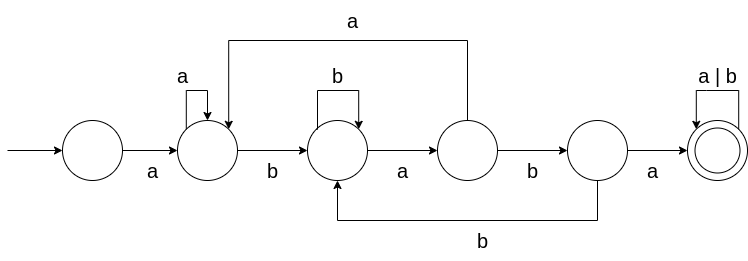
\includegraphics[width=1\textwidth]{hw1-dfa3a.png}
    \end{figure}

    \subsection*{3b}
    \verb!(01|1)*(0|!$\epsilon$\verb!)111(01|1)*(0|!$\epsilon$\verb!)! \\

    To construct the regular expression, we begin with $111$ substring. Then we need to find a regular expression that describes any string of $0$ and $1$ but does not contain $00$ as a substring. If we add this regular expression before and after $111$ substring, we should have a complete description of the language.

    To find the regular expression that does not produce $00$ substring, we can say that if we start with $0$ then we need to follow it with a $1$, but a $1$ can stand on its own. So this leads to \verb!(01|1)*!. However, the drawback with this is that a single $0$ cannot stand on its own. So we add \verb!0|!$\epsilon$ as suffix resulting in \verb!(01|1)*(0|!$\epsilon$\verb!)!. Putting together all these pieces leads to the above complete regular expression for the language.

    The below DFA is a representation of the above regular expression. This DFS was derived using Thompson's construction, Subset construction and Hopcroft's algorithm.

    \begin{figure}[H]
        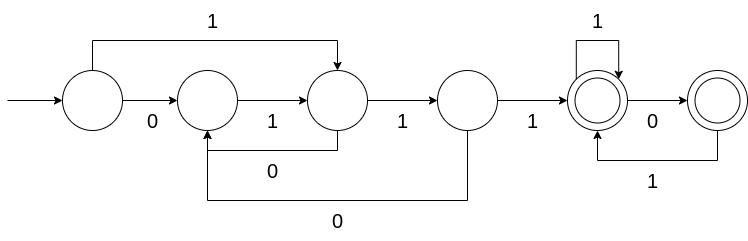
\includegraphics[width=1\textwidth]{hw1-dfa3b.png}
    \end{figure}

    \section*{Question 4}
    
    \subsection*{4a}
    \verb!Octal ::= 0[0-7]*! \\
    \verb!Decimal ::= [1-9][0-9]*! \\
    \verb!Hexadecimal ::= 0[xX][0-9a-fA-F]+! \\
    \verb!Unsigned ::= u|U! \\
    \verb!Long ::= l|L! \\
    \verb!Suffix ::= (Unsigned? Long?) | (Long? Unsigned?)! \\
    \verb!IntegerConstant ::+ (Octal | Decimal | Hexadecimal) Suffix?! \\

    We start with the definition of octal, decimal and hexadecimal as specified in the question. The suffix (if any) for unsigned and long can occur once and in any order, so we need to consider both possible orders. Putting this together leads to the above regular expression for integer constants.

    \subsection*{4b}
    \begin{figure}[H]
        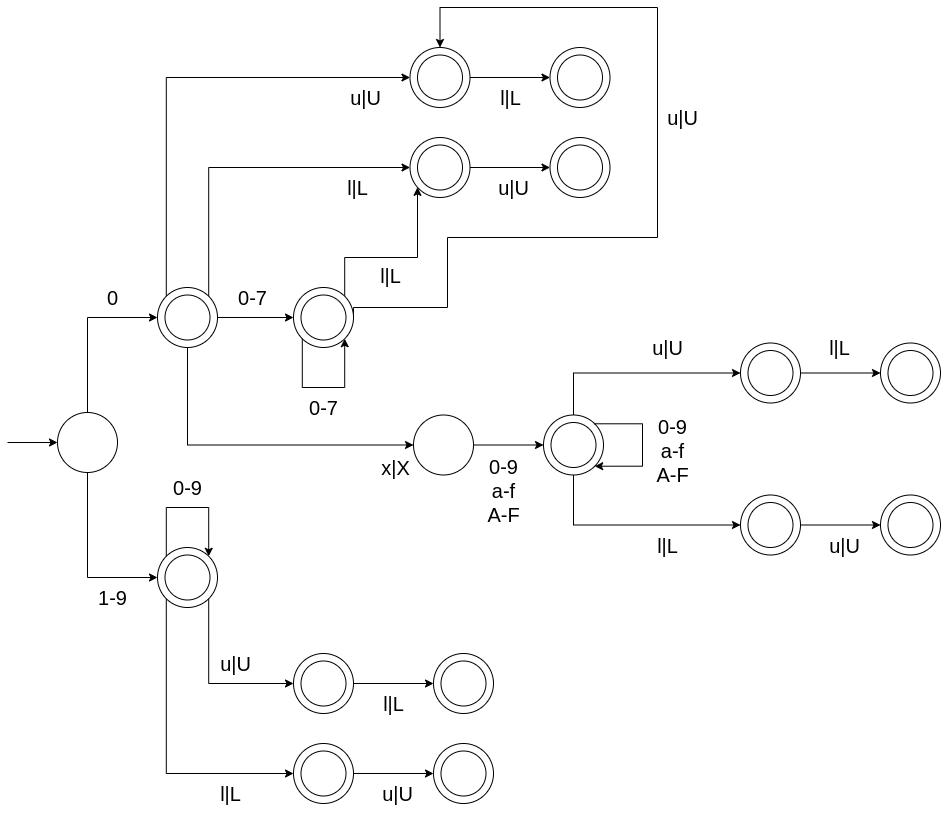
\includegraphics[width=1\textwidth]{hw1-dfa4b.png}
    \end{figure}


    \section*{Question 5}

    \subsection*{5a}
    \verb!CommentMiddle ::= ([^!$\underline{-}$\verb!])|(-[^!$\underline{-}$\verb!])|(---*[^>!$\underline{-}$\verb!])! \\
    \verb|HtmlComment ::= <!--CommentMiddle*--(-*)>| \\

    There is a well defined starting and ending character sequence for HTML comments. So focusing on the middle section of the comment, we form a regular expression that either allows all characters except $-$ or allows $-$ but not followed by $-$ or allows $--$ but not followed by $>$. But this does not cover a single $-$ which is a valid comment content. This is true for a multiple repetitions of $-$ as well. To cover this, we interpret the ending character sequence to allow two or more $-$ followed by $>$.

    \subsection*{5b}
    \begin{figure}[H]
        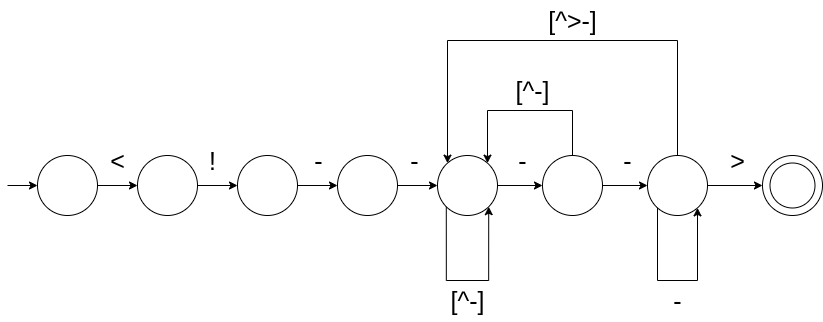
\includegraphics[width=1\textwidth]{hw1-dfa5b.png}
    \end{figure}

\end{document}
